\section{Sistemas de Información Geográfica}

Un \textit{sistema de información geográfica} (SIG) es un conjunto de herramientas que integra y relaciona diversos componentes que permiten la organización, almacenamiento, manipulación y análisis de grandes cantidades de datos procedentes del mundo real que están vinculados a una referencia espacial.

\vspace{3mm}

Para obtener la información que nos interesa de un mapa, como calles, coordenadas de esquinas, etc., debemos utilizar un servicio de geolocalización como \textit{Google Maps}. Sin embargo, este no nos proporciona toda la información que necesitamos, por lo tanto, usaremos \textit{Open Street Map (OSM)}, un proyecto colaborativo de origen británico para crear mapas editables y libres.

\vspace{3mm}

Dado que las zonas de San Isidro no son rectángulos, más bien son polígonos, tuvimos que generar primero estas figuras utilizando archivos \textit{geojson}, los cuales son archivos \textit{json} con una estructura predefinida específica para contextos geográficos. Por otro lado, no queremos únicamente el polígono de la zona a recorrer, si no que también queremos los alrededores para poder darle la posibilidad al camión de salir de la zona y volver a entrar simulando movimientos permitidos en la realidad. Con lo cual, tendríamos un polígono extendido ligado a una zona, el cual contiene la zona y sus alrededores. Luego a través de una API brindada por \textit{OSM} podemos obtener el mapa con todos los detalles del polígono utilizado.

\section{Transformando Mapas en Grafos}

Una vez generado el mapa \textit{OSM} vamos a querer manipularlo para poder retener únicamente la información que nos importa y agregarle datos adicionales que no se encuentran en \textit{Open Street Maps} que nos brindaron del Municipio. Resumiendo, de cada calle queremos saber si:
\begin{itemize}
    \item Estamos obligados a recorrerla recolectando residuos.
    \item Si es mano única o doble.
    \item Forma parte de un barrio privado o informal.
    \item Si es una calle de empedrado.
    \item Si una de sus esquinas es un cruce ferroviario.
    \item Si una de sus esquinas tiene un semáforo y si este tiene giro a la izquierda.
\end{itemize}

Para ello vamos a filtrar el mapa \textit{OSM} quedándonos con los elementos que tienen cierto \textit{keyword} identificándolos como una calle para poder generar el grafo mixto $G$ modelando las intersecciones como nodos y las calles como aristas. Por lo tanto, generaríamos un grafo $G = (V, E \cup A)$ donde $E$ es el conjunto de aristas y $A$ el conjunto de arcos.

\vspace{3mm} 

Sea $C$ el conjunto de calles del mapa \textit{OSM}. El proceso para filtrar el mapa se basa en analizar cada $c\in C$, para ello comenzamos separando en obligatorias o no usando la librearía de python, \textit{shapley}, con la cual podemos verificar si un punto está dentro de un polígono en el mapa. Luego, conociendo las esquinas de la calle $c$ que estamos analizando las vamos a agregar al conjunto de nodos $V$ marcando si tiene alguna característica de interés como cruce de tren, semáforo con o sin luz de giro, etc. 

\vspace{3mm}
Para realizar esta decisión debemos comparar coordenadas, ya que es la única información en común entre las esquinas del mapa \textit{OSM} y el dataset brindado por el municipio. Luego, dada una lista de puntos $A$ y una esquina candidata $e$, queremos determinar si existe $a \in A$ tal que $e$ corresponda al mismo punto que $a$.

\vspace{3mm}

Para verificar si dos coordenadas representan la misma esquina utilizamos la distancia euclídea, considerando que $|a - e|_2 < \epsilon$. No buscamos igualdad exacta ya que, al tratarse de coordenadas geográficas, pueden existir pequeñas diferencias en su representación para una misma esquina en distintos mapas o datasets.

\vspace{3mm}

Para resolver este pequeño problema vamos a pensar la lista de coordenadas como una matriz $A$ donde cada fila es una coordenada del dataset. A cada fila le vamos a restar el punto $e$ generando una matriz $A'$.Luego, siendo $A'_i$ la $i$-ésima fila de $A'$, vamos a corroborar que $\min_{i=1,\dots,n}(\|A'_i\|_2) < \epsilon$. 

Esta operación puede implementarse de manera muy eficiente utilizando \textit{NumPy}, ya que la resta del punto $e$ a todas las filas de la matriz y el cálculo de las normas pueden realizarse mediante operaciones vectorizadas. Estas permiten aplicar una misma operación a todos los elementos de un arreglo de manera simultánea, evitando iteraciones explícitas y aprovechando implementaciones optimizadas de bajo nivel.

\vspace{3mm} 

Una vez filtrado el mapa vamos a eliminar las calles que no podemos recorrer. Estas calles son las que no tienen salida, ya que el camión no puede dar un giro en U en este tipo de calles. Para ello vamos a eliminar los nodos tal que pertenezcan a alguno de los siguiente 3 conjuntos, una vez eliminados, vamos a volver a generar estos conjuntos y repetir el proceso hasta que al volverlos a generar estén los 3 vacíos.

\begin{itemize}
    \item $I = \{v\in V: d^+(v) = 0\}$
    \item $O = \{v\in V: d^-(v) = 0\}$
    \item $U = \{v\in V: d^+(v) = d^-(v) = 1 \land \exists u\in V : uv,vu \in E\}$
\end{itemize}

El conjunto $I$ representa las intersecciones inaccesible para nosotros, generado en consecuencia de que estamos tomando un polígono el cual deja calles afuera, en particular, calles que conectan puntos fuera del polígono con los que están dentro. Luego, el conjunto $O$ representa intersecciones parecidas a las de $I$, salvo que son para el otro sentido, es decir, son las que conectan puntos de nuestro polígono con los puntos fuera de el. Finalmente, el conjunto $U$ son las verdaderas calles sin salida que se encuentran en la ciudad.

\vspace{3mm} 

El siguiente paso es calcular los costos de cada arista o arco, tiempo, dist, demanda...

\vspace{3mm} 

Otro dato de interés son las curvas, ya que queremos minimizar la cantidad de curvas tomadas por el camión. Para identificar las curvas vamos a utilizar los nombres de cada calle, con lo cual, dadas 3 intersecciones, $u,v$ y $w$, estando parados en la intersección $v$, viniendo de la calle que une las intersecciones de $u$ a $v$, continuando por la calle que une $v$ y $w$, vamos a marcar como curva el recorrido $uvw$ si y sólo si los nombres de las calles que unen las intersecciones difieren.
\vspace{3mm} 

Continuando con las curvas, además de marcarlas, vamos a identificar cuales son curvas a la izquierda y si están prohibidas. Para ello, vamos a analizar las triplas para las cuales la calle que une la intersecciones $u$ y $v$ es doble mano o una avenida sin semáforo para girar a la izquierda. Una vez tenemos el conjunto de candidatas, vamos a calcular el ángulo orientado en sentido horario que generan y si este este pertenece al intervalo $[\textit{threshold} \pi]$ lo consideraremos como un giro a la izquierda ilegal.

\vspace{3mm} 

En la siguiente figura podemos visualizar el mapa \textit{OSM} filtrado, donde las calles de color \textit{amarillo} son las calles obligatorias de recorrer, las \textit{azules} son las calles empedradas y las \textit{grises} son las no obligatorias.


\begin{figure}[h!]
    \centering
    \begin{minipage}{0.48\textwidth}
        \centering
        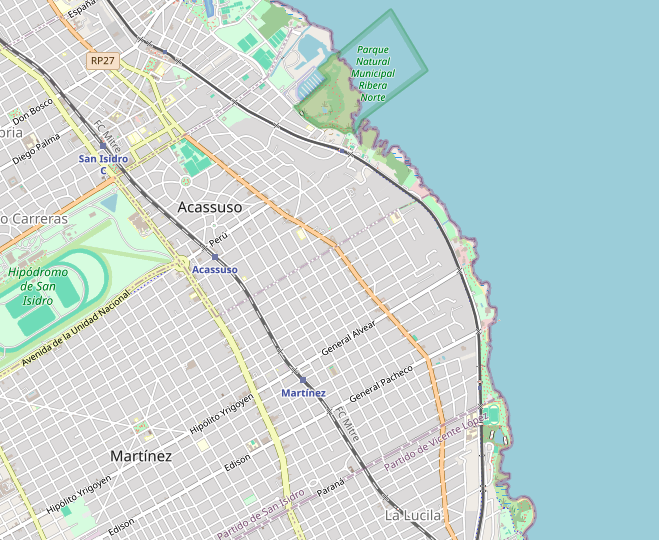
\includegraphics[width=\textwidth]{img/AcassusoReal.png}
        \caption{Acassuso \textit{OSM}}
        \label{fig:imagen1}
    \end{minipage}
    \hfill
    \begin{minipage}{0.48\textwidth}
        \centering
        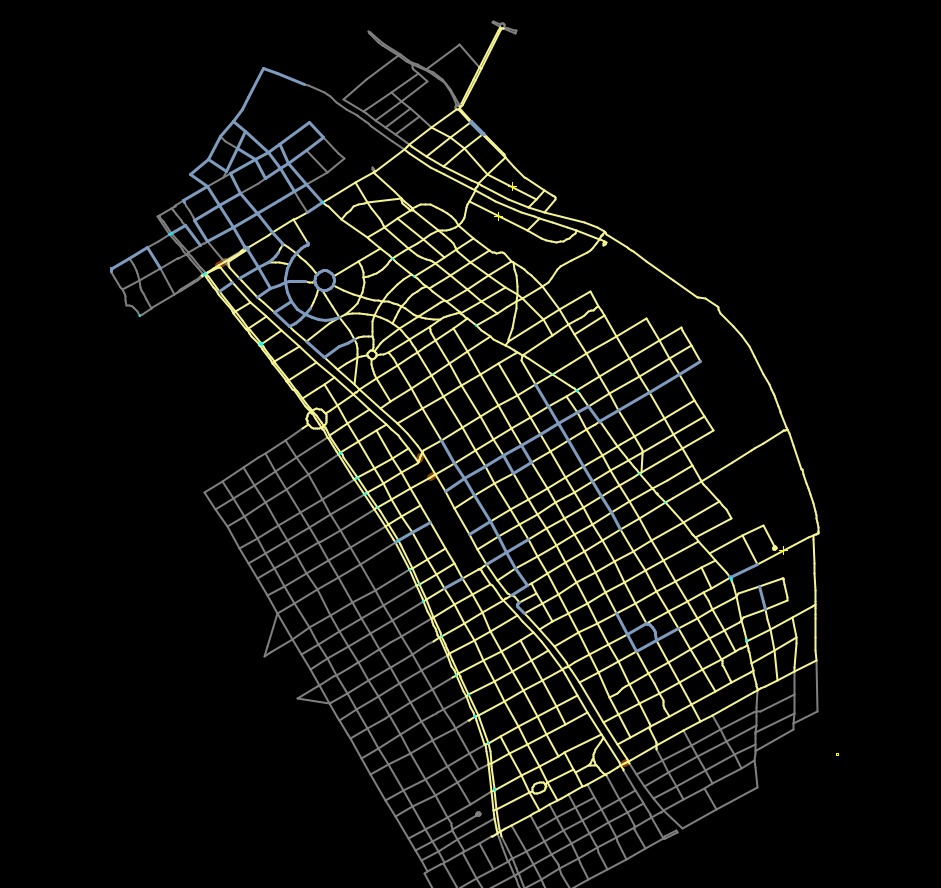
\includegraphics[width=\textwidth]{img/AcassusoOSM.jpeg}
        \caption{Acassuso \textit{OSM} Filtrado}
        \label{fig:imagen2}
    \end{minipage}
\end{figure}

Recapitulando, a partir de un polígono generamos un una instancia del problema donde tenemos el grafo $G = (V, E\cup A)$, es decir el área a recolectar, y 2 funciones $t:E\cup A\rightarrow \mathbb{R}$ y $d:E\cup A\rightarrow \mathbb{R}$ que representan, para todo eje perteneciente a $G$, el costo en tiempo (seg) de recorrerlo y la demanda de basura del mismo respectivamente.


\subsection{Zonificando con Grillas}

Para poder zonificar el grafo en $k$ debemos procesar el mapa como fue explicado anteriormente. En un principio, no tuvimos problemas con el modelo, sin embargo, a medida que lo fuimos probando con instancias reales, el modelo comenzó a demorar mucho más de lo esperado. El objetivo de la zonificación era obtener un resultado concreto y rápido para que luego el modelo de optimización de recorridos encuentre la solución óptima.

\vspace{3mm}

Llegamos a la conclusión que estábamos entrando muy en detalle utilizando todos las intersecciones y calles del área para asignarles una zona. Para este problema auxiliar no queríamos una solución óptima de la distribución de calles, necesitábamos una solución eficaz y eficiente. Por lo tanto, decidimos separar el mapa en una grilla, donde cada celda contendría un conjunto de calles e intersecciones y representaría un nodo en el modelo, reduciendo los nodos un 98$\%$ y las aristas un 93$\%$ en promedio. [CHEQUEAR PORCENTAJES] 

\vspace{3mm}

El primer paso para generar la grilla es tomar las coordenadas extremas en latitud y longitud. A partir de este paso ya tenemos una grilla que contiene todos los nodos y aristas del grafo. Sin embargo, como el mundo no es perfecto, las calles de nuestra ciudad no están perfectamente alineadas con la latitud o la longitud, con lo cual, vamos a tener que rotar la grilla.

\vspace{3mm}

Para poder rotar la grilla necesitamos tener un ángulo de rotación, para ello, necesitamos formar un triangulo en nuestro mapa, donde el \textcolor{blue}{hipotenusa} quede alineado con una calle seleccionada previamente para alinear la grilla y el \textcolor{green!50!black}{cateto 2} paralelo a la longitud. Una vez generado el triángulo basta obtener el ángulo entre el \textcolor{red}{cateto 1} y la \textcolor{blue}{hipotenusa} para saber cuanto necesitamos girar la grilla. Una vez que tenemos el ángulo vamos a utilizar el método de \textbf{Givens} usado para rotar matrices $4\times4$ para rotar nuestra grilla y alinearla a las calles de la zona.

[DECIR QUE LA DISTANCIA SE CALCULA DE OTRA MANERA EN LA TIERRA?]

\begin{figure}[h!]
    \centering
    \begin{minipage}{0.48\textwidth}
        \centering
        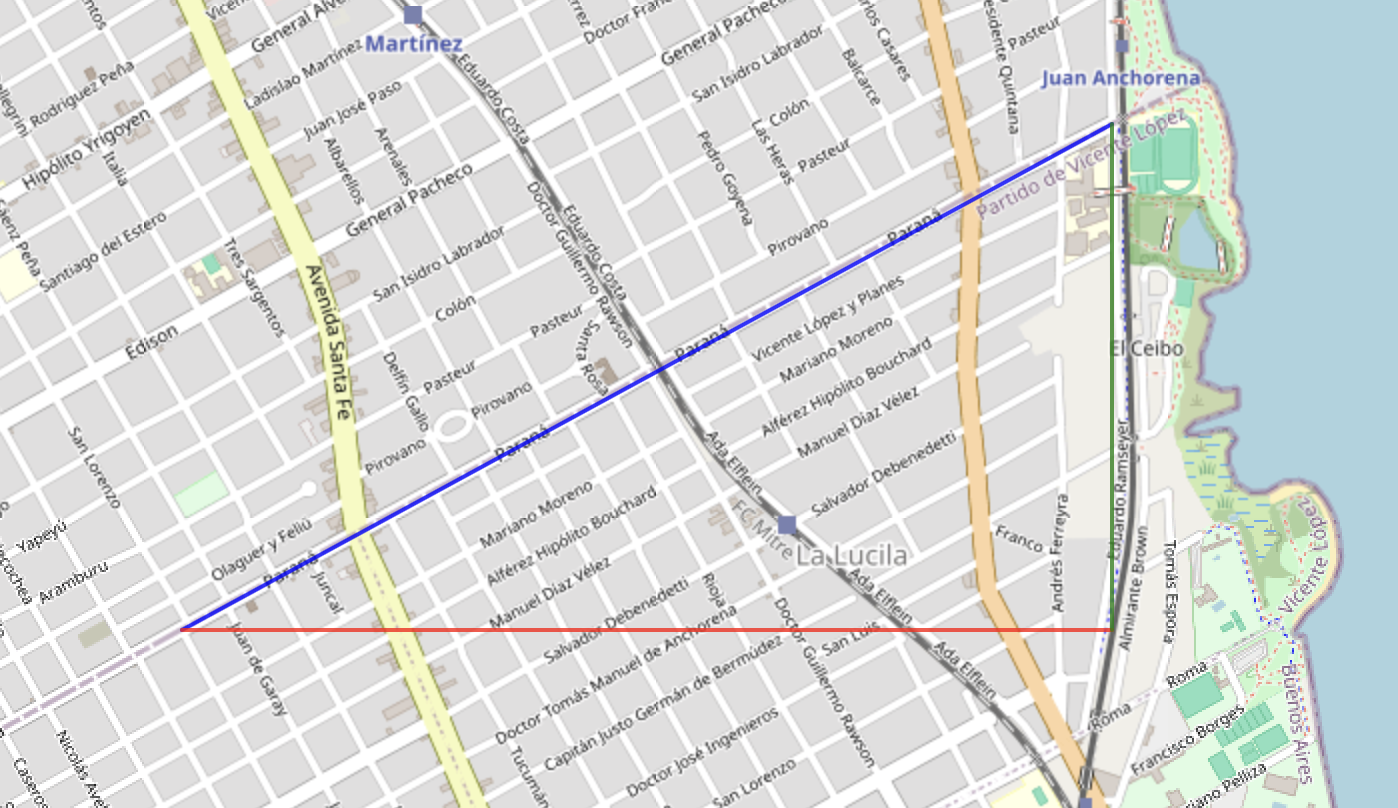
\includegraphics[width=\textwidth]{img/triangulo.png}
        \caption{Triángulo de rotación}
        \label{fig:triangulo}
    \end{minipage}
    \hfill
    \begin{minipage}{0.48\textwidth}
        \centering
        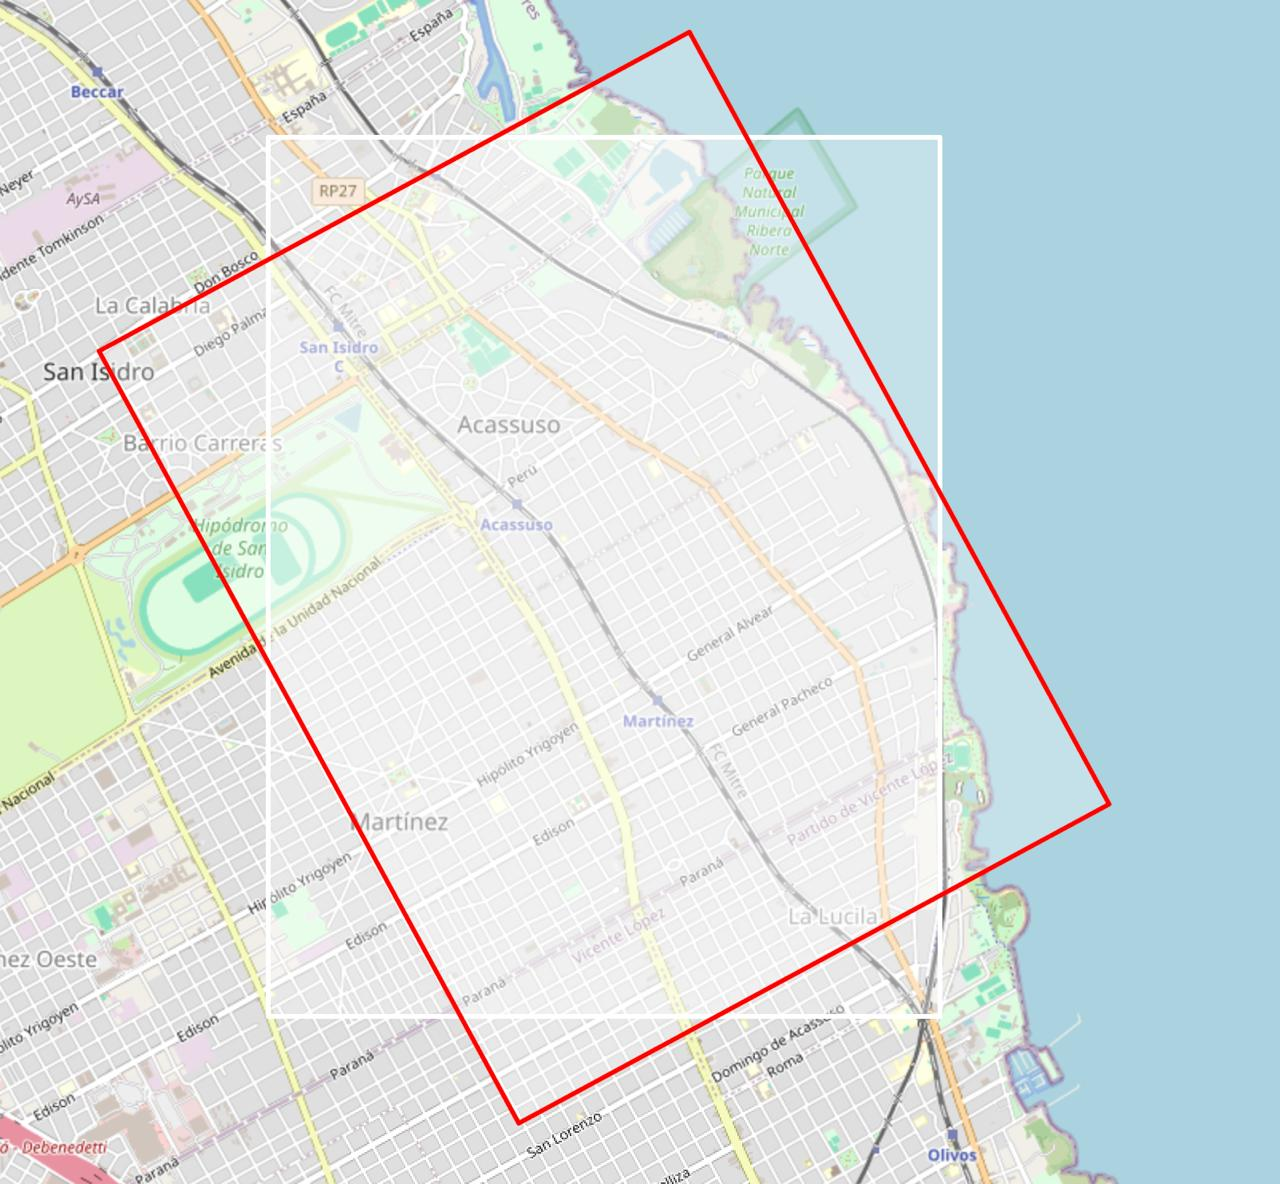
\includegraphics[width=\textwidth]{img/grilla_rotada.jpeg}
        \caption{\textcolor{red}{Grilla rotada} vs Grilla original}
        \label{fig:imagen2}
    \end{minipage}
\end{figure}


El siguiente paso es generar las celdas, para ello, a través de un parámetro externo sobre la máxima cantidad de celdas, dividimos equitativamente la grilla para obtener lo más parecido a este parámetro. Luego, debemos iterar celda por celda para poder calcular la demanda de cada una de ellas con la siguiente fórmula:
$$
D(C) = \sum_{(u,v) \in E \space \land \space (u,v) \in C} d((u,v))
$$

Esto se traduce a decir que la demanda $D$ de cada celda $C$ es la sumatoria de la demanda $d:E\rightarrow \mathbb{R}$ de toda arista $(u,v)$ que se encuentra dentro de la celda.

\vspace{3mm}

Finalmente obtuvimos una grilla la cual podemos traducir a un grafo grilla con demanda por nodo y distancia entre ellos calculada desde el centro de cada grilla.

